%%%%%%%%%%%%%%%%%%%%%%%%%%%%%%%%%%%%%%%%%
% Short Sectioned Assignment
% LaTeX Template
% Version 1.0 (5/5/12)
%
% This template has been downloaded from:
% http://www.LaTeXTemplates.com
%
% Original author:
% Frits Wenneker (http://www.howtotex.com)
%
% License:
% CC BY-NC-SA 3.0 (http://creativecommons.org/licenses/by-nc-sa/3.0/)
%
%%%%%%%%%%%%%%%%%%%%%%%%%%%%%%%%%%%%%%%%%

%----------------------------------------------------------------------------------------
%	PACKAGES AND OTHER DOCUMENT CONFIGURATIONS
%----------------------------------------------------------------------------------------

\documentclass[paper=a4, fontsize=11pt]{scrartcl} % A4 paper and 11pt font size

\usepackage[T1]{fontenc} % Use 8-bit encoding that has 256 glyphs
\usepackage{fourier} % Use the Adobe Utopia font for the document - comment this line to return to the LaTeX default
\usepackage[english]{babel} % English language/hyphenation
\usepackage{amsmath,amsfonts,amsthm} % Math packages

\usepackage{lipsum} % Used for inserting dummy 'Lorem ipsum' text into the template

\usepackage{sectsty} % Allows customizing section commands
\allsectionsfont{\centering \normalfont\scshape} % Make all sections centered, the default font and small caps

\usepackage{tikz}
\usetikzlibrary{plotmarks}

\usepackage{enumitem}
\usepackage{lastpage}
\usepackage{multirow}
\usepackage{fancyhdr} % Custom headers and footers
\pagestyle{fancyplain} % Makes all pages in the document conform to the custom headers and footers
\fancyhead{} % No page header - if you want one, create it in the same way as the footers below
\fancyfoot[L]{} % Empty left footer
\fancyfoot[C]{} % Empty center footer
\fancyfoot[C]{\thepage~of~\pageref{LastPage}} % Page numbering for right footer
\renewcommand{\headrulewidth}{0pt} % Remove header underlines
\renewcommand{\footrulewidth}{0pt} % Remove footer underlines
\setlength{\headheight}{13.6pt} % Customize the height of the header

\setlength\parindent{0pt} % Removes all indentation from paragraphs - comment this line for an assignment with lots of text

%----------------------------------------------------------------------------------------
%	TITLE SECTION
%----------------------------------------------------------------------------------------

\newcommand{\horrule}[1]{\rule{\linewidth}{#1}} % Create horizontal rule command with 1 argument of height



\title{	
\normalfont \normalsize 
\textsc{Norwegian University of Science and Technology\\TDT4200 -- Parallel Computing} \\ [25pt]
\horrule{0.5pt} \\[0.4cm]
\huge Problem Set 1:\\ MPI Intro\\
\horrule{2pt} \\[0.5cm]
}

\author{Per Magnus Veierland\\permve@stud.ntnu.no}

\setlist[enumerate,1]{label=\emph{\alph*})}
\setlist[enumerate,2]{label=\roman*)}
\setlist[enumerate,3]{label=\arabic*)}

\date{\normalsize\today}

\newacro{ALU}{Arithmetic Logic Unit}
\newacro{MIMD}{Multiple instruction-stream, multiple data-stream}
\newacro{MISD}{Multiple instruction-stream, single data-stream}
\newacro{MPI}{Message Passing Interface}
\newacro{SIMD}{Single instruction-stream, multiple data-stream}
\newacro{SISD}{Single instruction, single data-stream}
\newacro{SSE}{Streaming SIMD Extensions}

\begin{filecontents}{div_soft.data}
#MOPS   Power [mW]
1.33E-02    10.403432
1.33E-01    12.53108
2.66E-01    14.90265
3.99E-01    17.22483
5.31E-01    19.58292
6.64E-01    21.89876
7.97E-01    24.44624
9.30E-01    26.6708
\end{filecontents}

\begin{document}
\maketitle

\section*{Part 1: Theory}

\subsection*{Problem 1: General Theory}

\begin{enumerate}

\item \textbf{Write a table explaining Flynn's Taxonomy.}

Flynn's taxonomy is a popular system used to categorize and describe computer architectures according to the number of instruction streams and data streams the system can operate on simultaneously.

\begin{itemize}

\item \textit{\acf {SISD}} refers to a classical and commonly used computer architecture in which there is a single stream of instructions being executed by the processor on a single stream of data fetched from memory. Conceptually this means that the processor has a single control unit and a single \ac{ALU}.

\item \textit{\acf{MISD}} refers to a computer architecture which conceptually has multiple control units and a single \ac{ALU}, i.e. it performs multiple instructions on the same set of data. This is an uncommon and little used configuration, but can be used in systems built for fault-tolerance where instructions can be computed redundantly and the results compared against each other to verify correctness. \\

\item \textit{\acf{SIMD}} refers to a computer architecture which conceptually has a single control unit and multiple \acp{ALU}. This means that the processor can execute single instructions which operate on multiple sets of data and can be found in almost all desktop processors with instruction sets additions such as \ac{SSE}.

\item \textit{\acf{MIMD}} refers to a computer architecture which conceptually has multiple control units and multiple \acp{ALU}. This refers to full hardware parallelism where multiple instruction streams are executed concurrently with separate data streams. The two common types of \ac{MIMD} systems which are \textit{shared-memory systems} in which multiple processor cores shares a common memory, and \textit{distributed-memory systems} where multiple pairs of processors with individual memories communicate via some interconnect.

\end{itemize}

\begin{enumerate}

\item \textbf{Explain how, where, and why MPI fits into Flynn's Taxonomy, and why if not.}

The \acf{MPI} library enables coordination of- and communication between separate programs running on separate data on separate computing nodes. In terms of Flynn's taxonomy this would make \ac{MPI} a \ac{MIMD} architecture assuming that the underlying system hardware is able to operate on multiple instruction- and data-stream simultaneously.

\end{enumerate}

\item \textbf{Shared Memory}

\begin{enumerate}

\item \textbf{Explain how and why (and why if not), MPI fits with Shared Memory systems.}

\end{enumerate}

\item \textbf{Distributed Memory}

\begin{enumerate}

\item \textbf{Explain how and why (and why if not), MPI fits with Distributed Memory systems.}

\end{enumerate}

\end{enumerate}

\subsection*{Problem 2: Code Theory}

\begin{enumerate}

\item \textbf{Does your implementation have any communicational bottlenecks?}

\begin{enumerate}

\item \textbf{Briefly outline the communicational bottleneck(s), if any.}

When implemented naively with one master node and $P-1$ slave nodes each slave node will compute its result and send it to the master through a single send and a single receive. This results in the master having to perform $P-1$ sequential receive calls to receive the results from all slaves. This bottleneck will only get worse as the number of nodes increases and in addition to increasing the time it takes to compute the final result it wastes CPU time by having slave programs stall while attempting to perform a blocking send to the master node.

\item \textbf{Is it possible to reduce the bottleneck, and if so how?}

This communicational bottleneck can be reduced by using tree-structured communication where the results are collected in branches towards the master through intermediary processing nodes. 

\begin{enumerate}

\item \textbf{If so, outline an algorithm that will reduce the bottleneck.}

With a branching factor of 2, processing nodes with an ID which is not a factor of 2 could communicate their result to the nearest lower processing node which has an ID which is a factor of 2. This could be repeated and the summed results from nodes with an ID factorable by 2 could be passed onto processing nodes which are factorable by 4 etc., until all results has reached the master node. Different branching factors can also be used. This reduces the communication bottleneck greatly by reducing the number of receives the master node must perform to $\log(P)$ and makes it scale much better with an increase in the number of processing nodes.

%A simple algorithm for each slave node to follow is:
%
%\begin{lstlisting}[language=C++]
%auto result = compute_node_result(processing_node_id);
%int i = processing_node_id;
%
%while (i != 0)
%{
%    if (i & 1)
%    {
%        send(i >> 1, result);
%        break;
%    }
%    else
%    {
%        auto received_result = receive_result_from_any_node();
%        result = combine_results(result, received_result);
%    }
%}
%\end{lstlisting}

\end{enumerate}

\end{enumerate}

\item \textbf{Does your implementation have any computational bottlenecks?}

\begin{enumerate}

\item \textbf{Briefly outline the computational bottleneck(s), if any.}

The computation task of the problem set is to compute the sum of a finite series of reciprocals of logarithms. The main components in computing this sum is a) a for-loop iterating the index, b) taking the logarithm of the index, c) a division calculating the reciprocal of the logarithm, d) adding the reciprocal of the logarithm to the sum. Among the elements of the total computation, benchmarking using Valgrind shows that more than 90\% of the naive program is spent on calculating logarithms which makes it the bottleneck of the computation.

\item \textbf{Is it possible to reduce the bottleneck(s)? If so, outline an algorithm/method that will reduce the bottleneck. A one line formula, if found, is acceptable (this is a hard question).}

There are several ways to significantly speed up the computation. Below are some of them listed.

\begin{itemize}

\item Since computing logarithms is expensive, reusing the results of computing them can provide great benefits by reducing the number of logarithm computations. The product rule of logarithms states that $\log_{b}(x*y)=\log_{b}(x) + \log_{b}(y)$. This rule means that by having the logarithms of the factors of a number, the logarithm of the number itself can be computed cheaply through additions. For any even number $X$ it is then sufficient to calculate the logarithm of $X/2$ and sum it with the logarithm of two, and likewise for increasing factors. An elegant way to compute as few logarithms as possible would be to use the Sieve of Eratosthenes (normally used to find prime numbers). With a sieve table logarithms of factors could be used optimally to find the logarithm of any number. An efficient way to use this technique while also splitting the program to run on several computing nodes was not found during the time available for this problem set.

A simpler algorithm was devised to reuse logarithms between a number $X$ and its double $2X$ which will always share the factor $2$. Starting with a range of numbers $[0,N]$ the range is split into 3: $[0,\frac{N}{4})$, $[\frac{N}{4},\frac{N}{2})$, $[\frac{N}{2},N)$. When calculating the logarithms for the numbers in the second range, the logarithms for all even numbers in the third range can be found at the same time since they will always share the factor two with the numbers in the second range. This algorithm can be applied recursively to the first range.

It can easily be seen that this algorithm will reduce the number of computed logarithms in the third range by a factor of 2. Since it is applied recursively to the first range it can be shown that the number of logarithmic computations saved is given by:

\begin{displaymath}
\sum\limits_{i=1}^{\infty} \bigg(\frac{1}{4}\bigg)^n = \frac{1}{3}
\end{displaymath}

This shows that reusing the logarithms for numbers sharing factors of two using this simple algorithm will reduce the total number of logarithms computed by $\frac{1}{3}$. Further improvements can be gained by reusing other common factors such as $3$ and $5$, but there may be limits to the value of reusing further factors as it also complicates the implementation.

Modifying the naive implementation to reuse logarithms for factors of two improved the running time from 3345391595 to 2364673326 nanoseconds which is an improvement of 29.32\%.

\item Computing natural logarithms is more expensive than computing logarithms with base 2. It is shown below that calculating the binary logarithm of $e$ divided by the binary logarithm of a number gives the same result as taking the reciprocal of the natural logarithm of the number. The average cost of computing one natural logarithm is 36 nanoseconds and the average cost of computing one binary logarithm is 28 nanoseconds. Since the value of $\log_{2}(e)$ can be precomputed once the change from computing natural logarithms to binary logarithms provides a speedup. When changing the naive implementation to use binary logarithms instead of natural logarithms the program went from spending 90.94\% of its running time on the logarithm function to spending 82.85\% of its running time on the logarithm function.

\begin{displaymath}
\frac{1}{\log_{e}(x)} = \frac{\log_{e}(e)}{\log_{e}(x)} = \frac{\log_{2}(e)}{\log_{2}(x)}
\end{displaymath}

\item The for-loop can be unrolled manually for an improvement in running time without complicating the program significantly. Unrolling the loop such that 8 terms are calculated per iteration instead of 1 reduced the running time of the naive implementation from $3408874911$ to $3370192981$ nanoseconds with $start=2$ and $stop=100000002$ which is an improvement of 1.13\%. After changing the naive implementation to use a binary logarithm instead of using a natural logarithm the program spend less time computing the logarithm and more time in the main program loop. Applying both the change from natural to binary logarithms and unrolling the loop by 8 reduced the running time from $3435538199$ to $2945741739$ nanoseconds which is an improvement of 14.26\%. Further small improvements could likely be made by spending more time tuning the unrolling.

\end{itemize}

\end{enumerate}

\end{enumerate}

\section*{Part 2: Code}

\subsection*{Problem 1: MPI Intro}

\begin{enumerate}

\item \textbf{In the MPI copy \texttt{computeMPI.c}, parallelize the serial program from \texttt{computeSerial.c} using MPI.}

\item \textbf{Implement a ``make all'' Makefile-rule which compiles and executes corresponding MPI file/executable in the given Makefile.}

\item \textbf{Analyze your implementation and report the following:}

\begin{enumerate}

\item \textbf{The amount of operations performed by your program as a function of $O(n)$, $n = stop - start$, and the amount of operations performed per process $\text{P}_\text{i}$ in your program with $i \in [1, 10]$.}

\item \textbf{The amount of MPI operations performed by your program as a function of $O(P)$, $P = NumberOfProcesses$.}

The program is split into one master process communicating with a set of slave processes. Each slave process will perform its computation based on the command line inputs and send one result to the master process using \texttt{MPI\_Send}. The number of slave processes is $P - 1$.

The master process will perform its own computation based on the command line inputs and then receive one result from each slave process using \texttt{MPI\_Recv}.

In total, the number of MPI operations performed by the program will be two times the number of slave processes; since each \texttt{MPI\_Send} from each slave process must be matched by one \texttt{MPI\_Recv} by the master process. Accordingly, $O(P) = P$.
$$\textit{NumberOfMpiOperations} = 2 * \textit{NumberOfSlaveProcesses} = 2 * (P - 1) = 2P - 2$$
$$O(P) = P$$

\item \textbf{The average amount of MPI operations performed per process $\text{P}_\text{i}$ in your program with $O(P)$, $P = NumberOfProcesses$.}

$(2P - 2) / P$

\item \textbf{The maximum number of MPI operations performed by any process $\text{P}_\text{i}$ as a function of $O(P)$, $P = NumberOfProcesses$.}

Will be by master node:
$P - 1$

\item \textbf{The difference in run-time with $P \in [1, 2, 4, 8]$ and $n = [2 \to 100, 2 \to 10^6, 2 \to 10^9]$ when run on a machine in ITS015.\\Make a graph for each value of P, showing the run-time for different increments of n. Each range of n should be split into 20 steps of equal increments.}

% format

% 4 graphs for each P



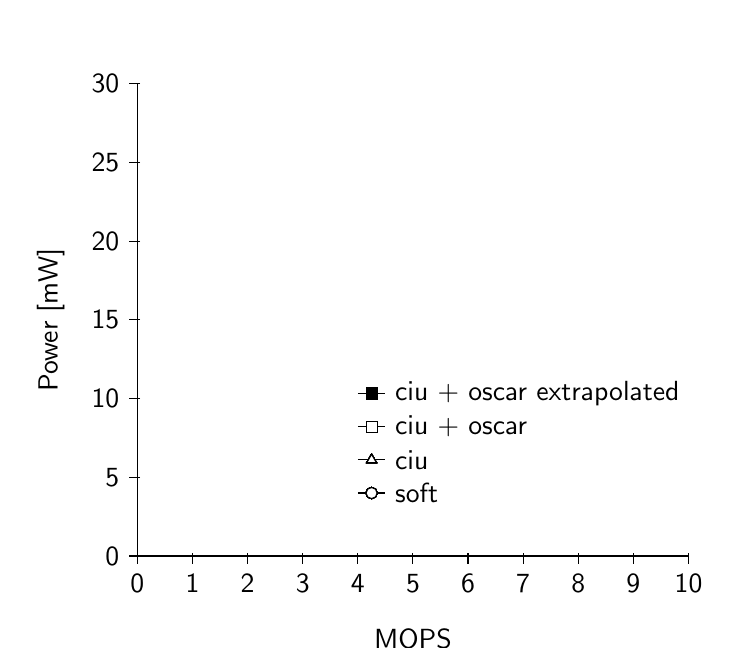
\begin{tikzpicture}[y=.2cm, x=.7cm,font=\sffamily]
%axis
\draw (0,0) -- coordinate (x axis mid) (10,0);
\draw (0,0) -- coordinate (y axis mid) (0,30);
%ticks
\foreach \x in {0,...,10}
\draw (\x,1pt) -- (\x,-3pt)
node[anchor=north] {\x};
\foreach \y in {0,5,...,30}
\draw (1pt,\y) -- (-3pt,\y) 
node[anchor=east] {\y}; 
%labels      
\node[below=0.8cm] at (x axis mid) {MOPS};
\node[rotate=90, above=0.8cm] at (y axis mid) {Power [mW]};

%plots
\draw plot[mark=*, mark options={fill=white}] 
file {div_soft.data};

%legend
\begin{scope}[shift={(4,4)}] 
\draw (0,0) -- 
plot[mark=*, mark options={fill=white}] (0.25,0) -- (0.5,0) 
node[right]{soft};
\draw[yshift=\baselineskip] (0,0) -- 
plot[mark=triangle*, mark options={fill=white}] (0.25,0) -- (0.5,0)
node[right]{ciu};
\draw[yshift=2\baselineskip] (0,0) -- 
plot[mark=square*, mark options={fill=white}] (0.25,0) -- (0.5,0)
node[right]{ciu + oscar};
\draw[yshift=3\baselineskip] (0,0) -- 
plot[mark=square*, mark options={fill=black}] (0.25,0) -- (0.5,0)
node[right]{ciu + oscar extrapolated};
\end{scope}
\end{tikzpicture}

\end{enumerate}

\end{enumerate}

\end{document}

